\documentclass[oneside,14pt]{extarticle}
\usepackage{cmap}
\usepackage[utf8]{inputenc}
\usepackage{longtable}
\usepackage[english,ukrainian]{babel}
\usepackage{graphicx}
\usepackage{geometry}
\usepackage{listings}
\usepackage{float}
\usepackage{amsmath}
\usepackage{subfig}
\usepackage{tempora}
\renewcommand{\arraystretch}{1.5}
\usepackage{mwe}
\geometry{
	a4paper,
	left=20mm,
	right=20mm,
	top=15mm,
	bottom=15mm,
}
\lstset{
	language=c,
	tabsize=4,
	keepspaces,
	showstringspaces=false,
	frame=single,
	breaklines,
	language=C,
}
\graphicspath{ {./pictures} }
\setlength{\parindent}{4em}

\newcommand\subject{Архітектура і проєктування програмного забезпечення}
\newcommand\lecturer{доцент кафедри ПЗ\\Фоменко А.В.}
\newcommand\teacher{старший викладач кафедри ПЗ\\Шкраб Р.Р.}
\newcommand\mygroup{ПЗ-42}
\newcommand\lab{5}
\newcommand\theme{Проектування системи за допомогою методології UML}
\newcommand\purpose{Вивчення основних принципів методології UML, створення Ознайомитися з технологією побудови UML-діаграм та побудувати їх}

\begin{document}
\begin{normalsize}
	\begin{titlepage}
		\thispagestyle{empty}
		\begin{center}
			\textbf{МІНІСТЕРСТВО ОСВІТИ І НАУКИ УКРАЇНИ\\
				НАЦІОНАЛЬНИЙ УНІВЕРСИТЕТ "ЛЬВІВСЬКА ПОЛІТЕХНІКА"}
		\end{center}
		\begin{flushright}
			\textbf{ІКНІ}\\
			Кафедра \textbf{ПЗ}
		\end{flushright}
		\vspace{80pt}
		\begin{center}
			\textbf{ЗВІТ}\\
			\vspace{10pt}
			до лабораторної роботи № \lab\\
			\textbf{на тему}: <<\textit{\theme}>>\\
			\textbf{з дисципліни}: <<\subject>>
		\end{center}
		\vspace{80pt}
		\begin{flushright}
			
			\textbf{Лектор}:\\
			\lecturer\\
			\vspace{28pt}
			\textbf{Виконав}:\\
			
			студенти групи \mygroup\\
			Коваленко Д.М.\\
			Снісар В.І.\\
			Баран В.Б.\\
			\vspace{28pt}
			\textbf{Прийняла}:\\
			
			\teacher\\
			
			\vspace{28pt}
			«\rule{1cm}{0.15mm}» \rule{1.5cm}{0.15mm} 2024 р.\\
			$\sum$ = \rule{1cm}{0.15mm}……………\\
			
		\end{flushright}
		\vspace{\fill}
		\begin{center}
			\textbf{Львів — 2024}
		\end{center}
	\end{titlepage}
		
	\begin{description}
		\item[Тема.] \theme.
		\item[Мета.] \purpose.
	\end{description}

    \section*{Лабораторне завдання}
    \begin{enumerate}
    	\item Постановка завдання. Необхідно описати постановку задачі виходячи з індивідуального завдання із зазначенням основних вимог до майбутньої системи та переліком її функціональності, повинна бути проведена структурна класифікація системи з метою визначення системних сутностей і їх стосунки між собою.
    	\item Представлення Use Case для системи з вказівкою акторів і вузлів. При виконанні даного етапу повинні бути побудовані діаграми Use Case, діаграма компонентів, діаграма кооперації, а також повинні бути подані відповідні опису акторів, вузлів і компонентів системи.
    	\item Діаграма послідовності, діаграма внутрішньої структури та діаграма основних класів системи.
    	\item Діаграму пакетів основних програмних сервісів системи і діаграма розгортання.
    	\item Обґрунтування вибору архітектури системи (тонкий або товстий клієнт), обґрунтування вибору середовища розробки, СУБД і операційної системи.
    	\item Прототип інтерфейсу. Повинні бути розроблені основні інтерфейси системи з урахуванням вимог до інтерфейсів. У звіті повинні бути представлені зображення інтерфейсів, які можна розробити в графічному або HTML редакторі або з використанням будь-якого середовища розробки програмного забезпечення. Основною вимогою до прототипу інтерфейсу є надання можливості представити як буде виглядати система в майбутньому.
    \end{enumerate}
    
    \section*{Хід роботи}
    \section{Концепція системи}
	\subsection{Опис проблемної області}
	У сучасному навчанні програмній інженерії студенти стикаються з необхідністю швидко освоювати методи проектування, зокрема використання UML-діаграм. Через обмеженість практичних ресурсів навчальні програми часто не мають спеціалізованих засобів для створення й аналізу діаграм, що відображають структуру, функціональність та взаємодію компонентів програмного забезпечення. Це призводить до браку практичного досвіду, що ускладнює процес навчання.
	
	\subsection{Постановка задачі}
	Завдання полягає у створенні Модуля проектування, що стане частиною «Віртуальної лабораторії програмної інженерії». Модуль повинен дозволяти студентам будувати UML-діаграми (варіантів використання, класів, послідовності) для моделювання архітектури та функціональності програмного забезпечення. Викладачі, у свою чергу, отримають можливість моніторити та оцінювати прогрес студентів на основі їхньої роботи з діаграмами.
	
	\subsection{Опис основного функціоналу системи}
	Модуль проектування включатиме такі ключові компоненти:
	\begin{itemize}
		\item Редактор діаграм варіантів використання: надає інструменти для створення акторів, варіантів використання та встановлення зв’язків між ними.
		\item Редактор діаграм класів: дозволяє додавати класи, їхні атрибути й методи, а також встановлювати зв’язки (наслідування, асоціації, композиції).
		\item Редактор діаграм послідовності: моделює взаємодію між об'єктами системи у вигляді послідовності повідомлень.
	\end{itemize}
	
	\subsection{Структурна класифікація системи}
	Модуль проектування складатиметься з таких підмодулів:
	\begin{enumerate}
		\item Підмодуль для діаграм варіантів використання;
		\item Підмодуль для діаграм класів;
		\item Підмодуль для діаграм послідовності;
		\item Інструмент валідації діаграм — для перевірки коректності побудови діаграм;
		\item Система збереження та експорту діаграм — забезпечує зберігання діаграм у базі даних та експорт у форматах JSON, XML.
	\end{enumerate}
	
	\subsection{Аналіз складності компонентів системи}
	\begin{itemize}
		\item Редактор діаграм: потребує створення гнучкого інтерфейсу з підтримкою drag-and-drop для елементів діаграм, що ускладнює розробку користувацького інтерфейсу.
		\item Валідація діаграм: розробка правил валідації, щоб запобігти логічним помилкам у діаграмах, потребує детального опрацювання.
		\item Експорт та збереження даних: забезпечення стабільного збереження даних і можливості їх експорту у різних форматах вимагає інтеграції з базами даних та налаштування механізмів конвертації.
	\end{itemize}
	
	\section{Архітектура системи}
	
	\subsection{Use Case діаграма}
	\begin{figure}[H]
		\centering
		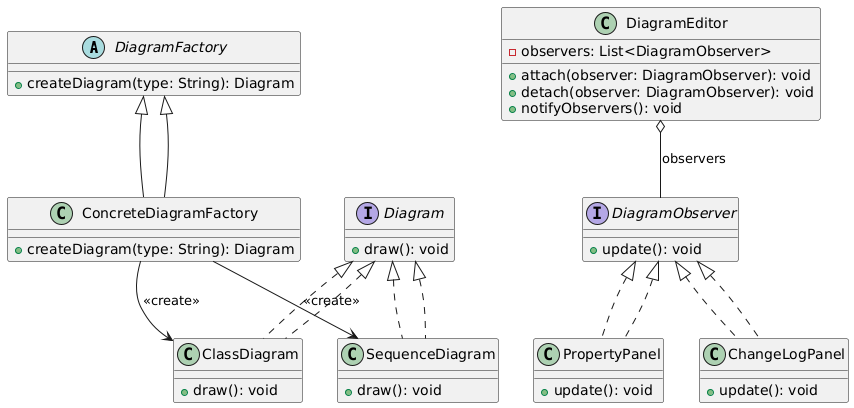
\includegraphics[width=\columnwidth]{1}
		\caption{Use Case діаграма}
	\end{figure}
	
	\subsection{Діаграма послідовності}
	\begin{figure}[H]
		\centering
		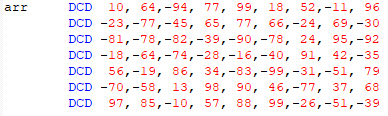
\includegraphics[width=\columnwidth]{2}
		\caption{Діаграма послідовності}
	\end{figure}
	
	\subsection{Діаграма кооперації}
	\begin{figure}[H]
		\centering
		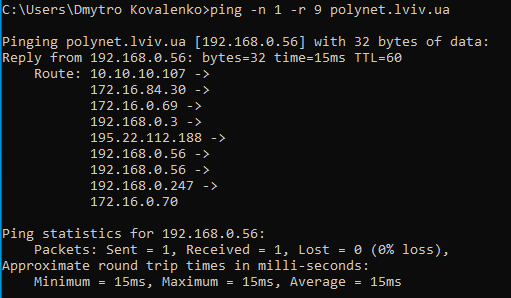
\includegraphics[width=\columnwidth]{3}
		\caption{Діаграма кооперації}
	\end{figure}
	
	\subsection{Діаграма діяльності}
	\begin{figure}[H]
		\centering
		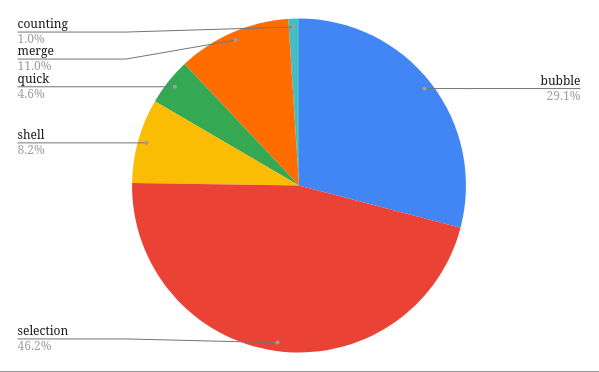
\includegraphics[width=\columnwidth]{4}
		\caption{Діаграма діяльності}
	\end{figure}
	
	\subsection{Діаграма основних класів системи}
	\begin{figure}[H]
		\centering
		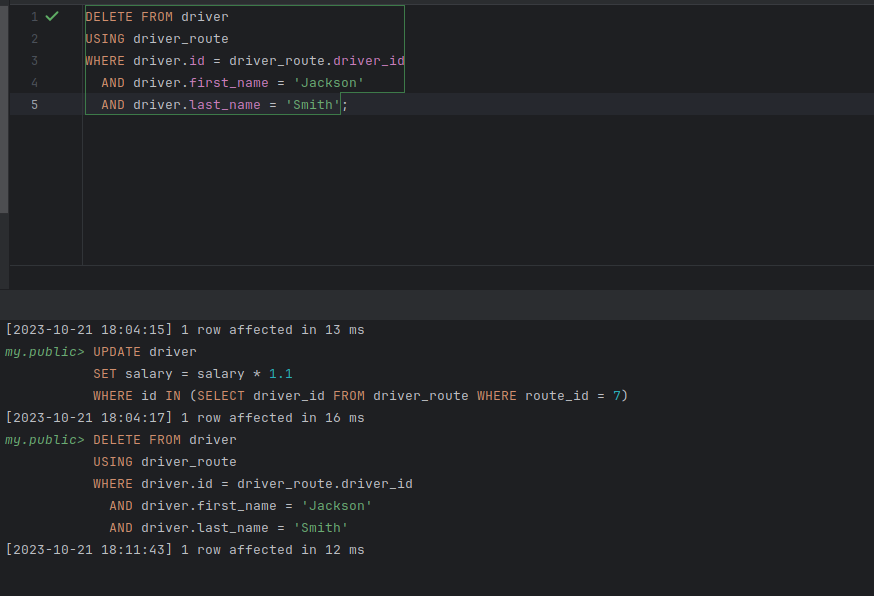
\includegraphics[width=\columnwidth]{5}
		\caption{Діаграма основних класів системи}
	\end{figure}
	
	\subsection{Діаграма об’єктів}
	\begin{figure}[H]
		\centering
		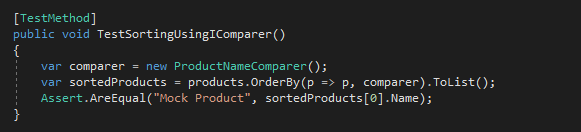
\includegraphics[width=\columnwidth]{6}
		\caption{Діаграма об’єктів}
	\end{figure}
	
	\subsection{Діаграма станів}
	\begin{figure}[H]
		\centering
		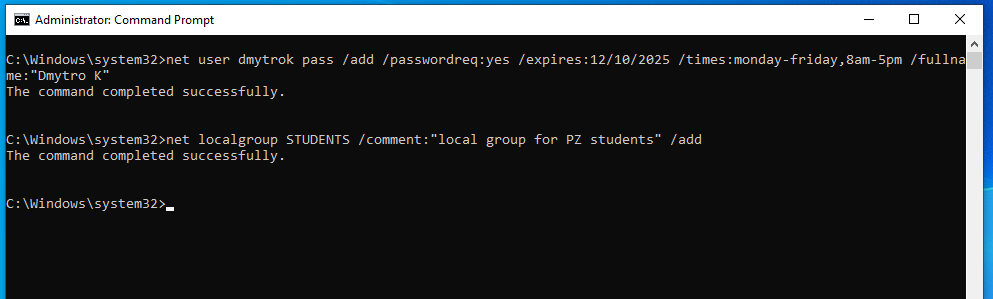
\includegraphics[width=\columnwidth]{7}
		\caption{Діаграма станів}
	\end{figure}
	
	\subsection{Діаграма пакетів}
	\begin{figure}[H]
		\centering
		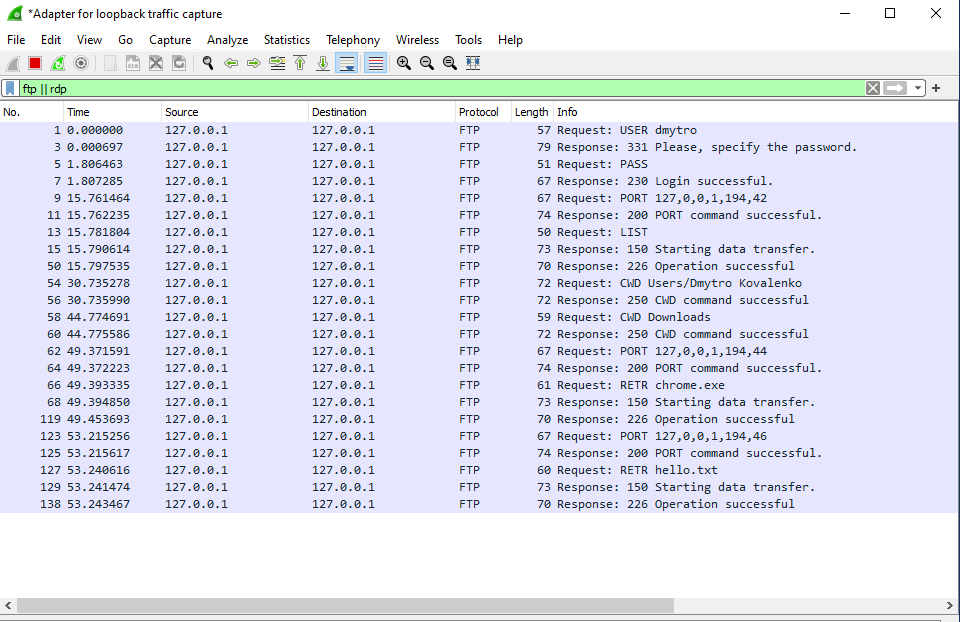
\includegraphics[width=\columnwidth]{8}
		\caption{Діаграма пакетів}
	\end{figure}
	
	\subsection{Діаграма компонентів}
	\begin{figure}[H]
		\centering
		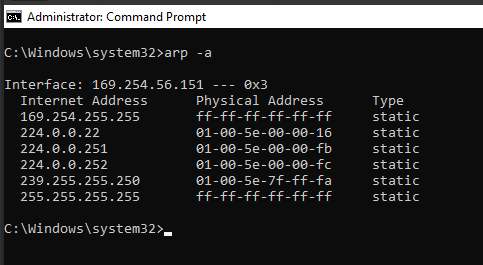
\includegraphics[width=\columnwidth]{9}
		\caption{Діаграма компонентів}
	\end{figure}
	
	\subsection{Діаграма внутрішньої структури}
	\begin{figure}[H]
		\centering
		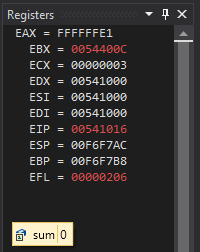
\includegraphics[width=\columnwidth]{10}
		\caption{Діаграма внутрішньої структури}
	\end{figure}
	
	\subsection{Діаграма розгортання}
	\begin{figure}[H]
		\centering
		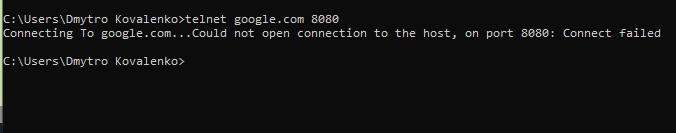
\includegraphics[width=\columnwidth]{11}
		\caption{Діаграма розгортання}
	\end{figure}
	
	\subsection{Вибір архітектури системи та обґрунтування технічних рішень}
	Для реалізації Модуля проектування обрано багаторівневу клієнт-серверну архітектуру з використанням шаблону Model-View-Controller (MVC). Розподіл на рівні забезпечує окреме опрацювання представлення (View), бізнес-логіки (Controller) та моделі даних (Model), що підвищує зручність у підтримці та масштабованості системи. Клієнтська частина виконує рендеринг інтерфейсу та обробляє взаємодію з користувачем, надсилаючи запити до серверної частини через REST API.
	
	На серверному рівні реалізовано сервісні класи для управління бізнес-логікою модуля, обробки даних діаграм та їх валідації. Така архітектура полегшує інтеграцію з іншими модулями «Віртуальної лабораторії», дозволяючи централізовано керувати доступом до даних та бізнес-процесами.
	
	\subsection{Обґрунтування вибору середовища розробки, СУБД і операційної системи}
	\begin{itemize}
		\item Середовище розробки: Intellij IDEA було обрано через його потужні засоби для розробки на Java та підтримку інтеграції з інструментами для UML-моделювання та базами даних. Це середовище також дозволяє легко налаштовувати плагіни, що спрощує налагодження та тестування коду.
		\item Система управління базами даних (СУБД): PostgreSQL є оптимальним вибором завдяки підтримці складних запитів та можливості зберігати JSON-об'єкти, що підходить для динамічного збереження даних діаграм. PostgreSQL забезпечує надійність, масштабованість та простоту інтеграції з іншими модулями.
		\item Операційна система: Ubuntu Server було обрано як операційну систему для серверної частини, оскільки вона надає стабільне та безпечне середовище з широкою підтримкою інструментів розробки та систем автоматизації.
	\end{itemize}
	
	\section{Архітектура системи}
	\subsection{Опис інтерфейсу користувача (mockups)}
	\begin{figure}[H]
		\centering
		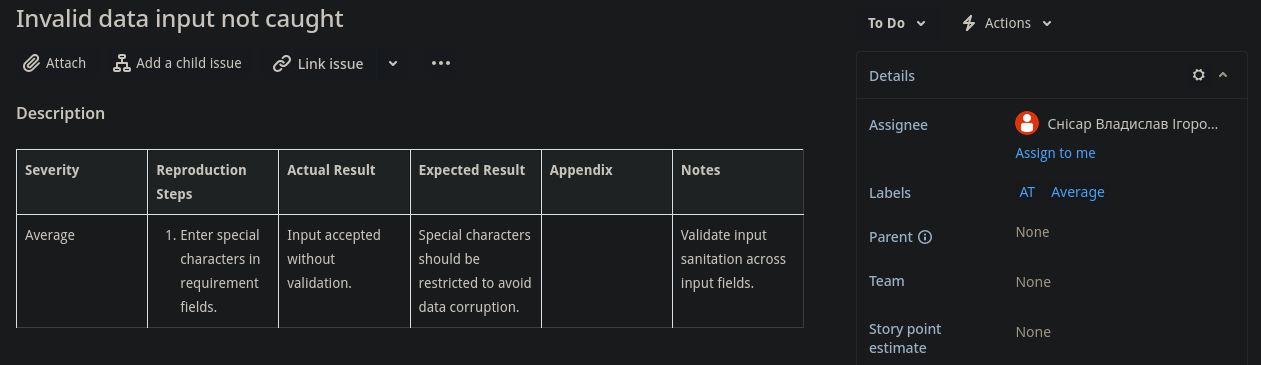
\includegraphics[width=\columnwidth]{13}
		\caption{Вікно реєстрації}
	\end{figure}
	
	\begin{figure}[H]
		\centering
		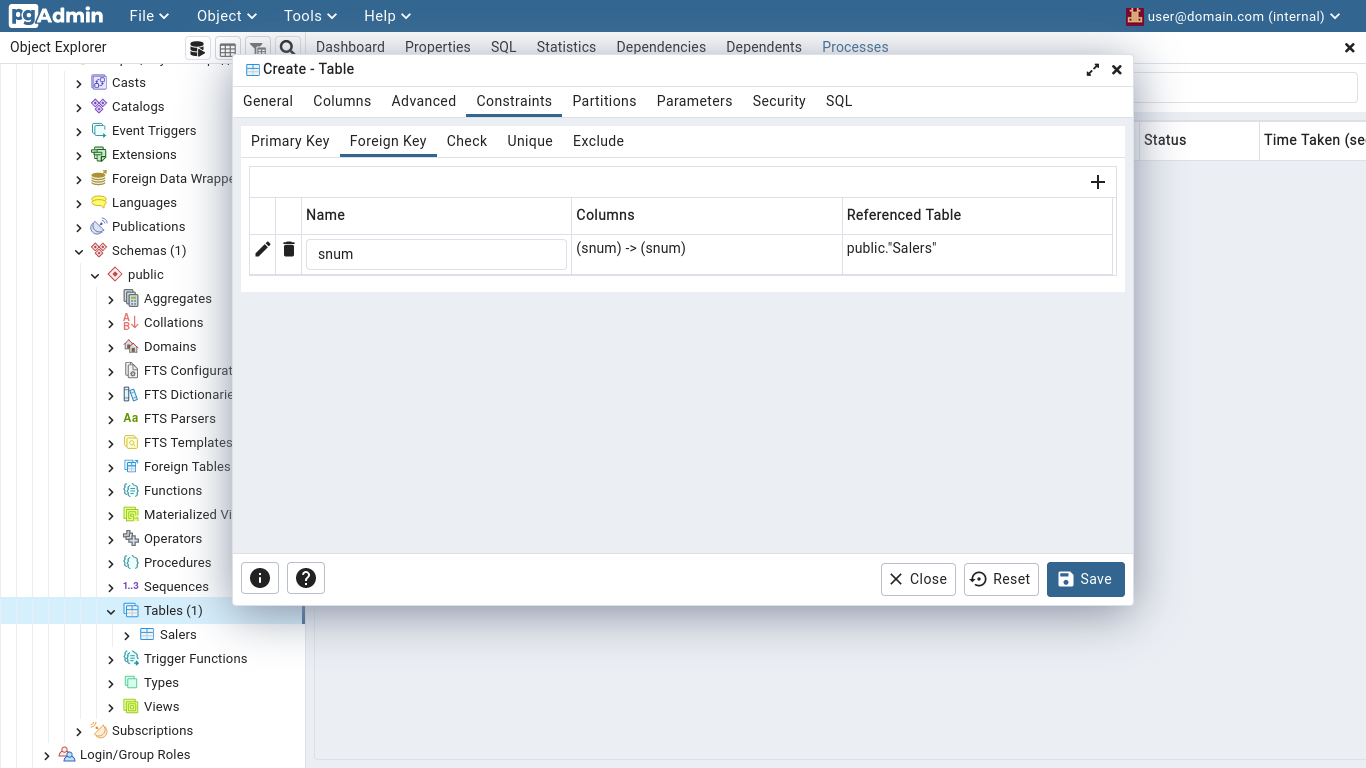
\includegraphics[width=\columnwidth]{12}
		\caption{Вікно редагування діаграм}
	\end{figure}
	
	\subsection{Основні компоненти інтерфейсу користувача – короткий огляд екранів і елементів GUI}
	\begin{figure}[H]
		\centering
		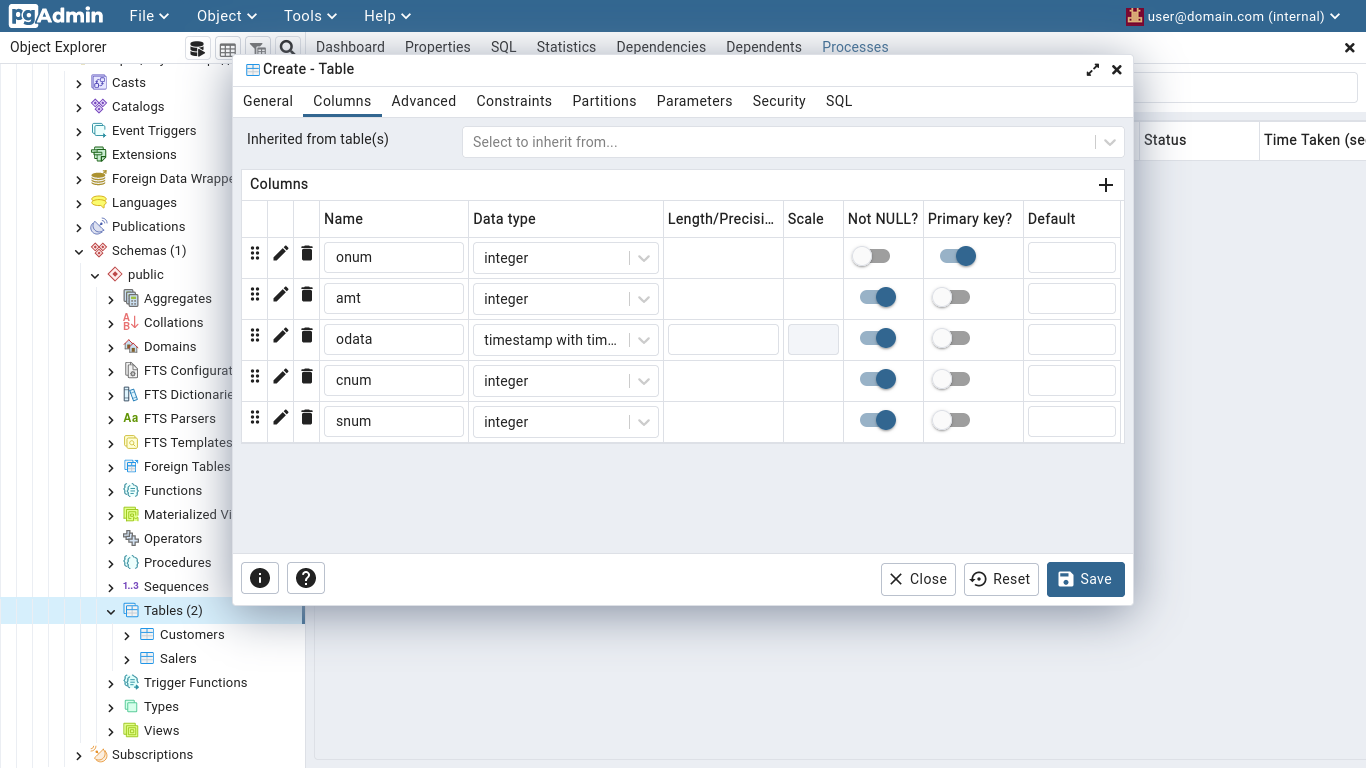
\includegraphics[width=0.3\columnwidth]{14}
		\caption{Елемент вибору компонентів діаграми}
	\end{figure}
	
	\begin{figure}[H]
		\centering
		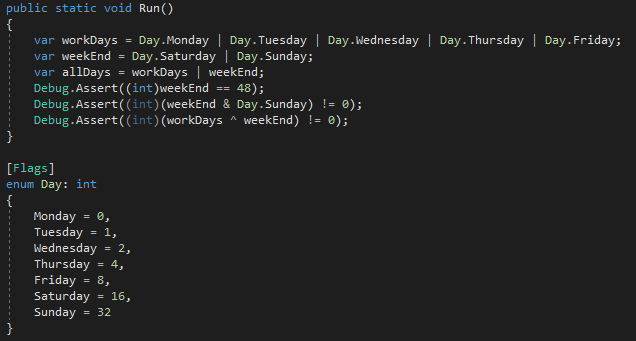
\includegraphics[width=\columnwidth]{15}
		\caption{Керування відображенням діаграми}
	\end{figure}
	
	\begin{figure}[H]
		\centering
		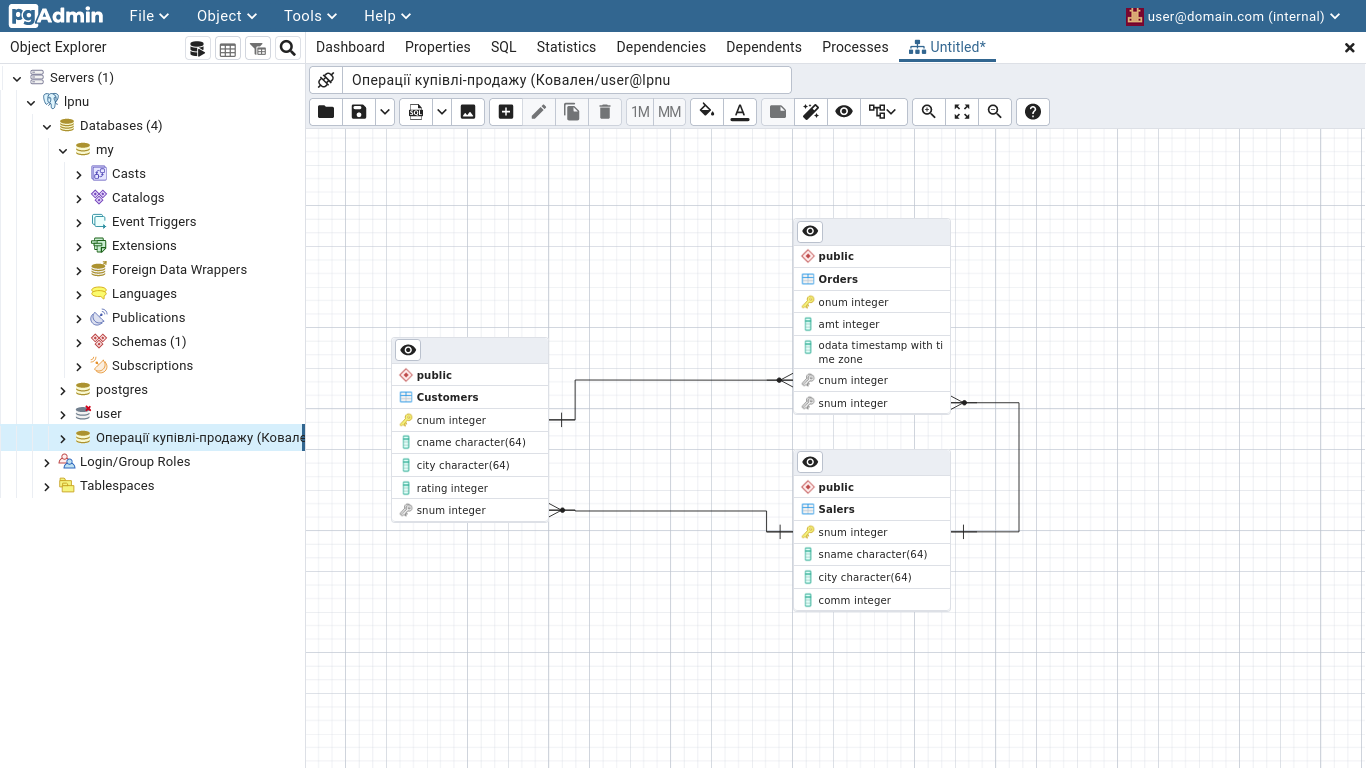
\includegraphics[width=\columnwidth]{16}
		\caption{Поле для редагування діаграми}
	\end{figure}
	
	\section*{Висновки}
	У результаті виконання лабораторної роботи було розроблено UML-діаграми до модуля пропозицій житла: use case діаграма, діаграми послідовності, кооперації, активності, класів, об’єктів, станів, внутрішньої структури, компонентів та розгортання. Діаграми описують модуль з різних точок зору і допомагають візуалізувати компоненти системи. Крім цього, було спроектовано мокапи системи, на основі яких буде створено інтерфейс.
	    
\end{normalsize}
\end{document}
